\documentclass[12pt]{article}

% 杂项宏包
\usepackage[colorlinks,linkcolor=blue]{hyperref}  % 超链接
\usepackage{amsmath}
\usepackage{amssymb}
\usepackage{multicol}
\usepackage{indentfirst}
\usepackage{algorithm}   % 代码块
\usepackage{algorithmicx}   % 代码块
\usepackage{algpseudocode}   % 代码块 
\usepackage{graphicx}  % 图片
\usepackage{subfigure}  % 并排图像
\usepackage{fontspec}
%\usepackage{parskip}
\usepackage[]{caption2}  % 去掉图表的冒号
\renewcommand{\captionlabeldelim}{}  % 去掉图表的冒号
\usepackage{booktabs} % 三线表
\usepackage{pdfpages}  % 直接插入pdf页面
\usepackage{caption}

% \setlength{\parindent}{2em}

% 字体设置
\usepackage{xeCJK}
%%%%%%%%%%% CJK下设置中文字体 %%%%%%%%%%%%%
\setCJKfamilyfont{song}{SimSun.ttf}
\newcommand{\song}{\CJKfamily{song}}
\setCJKfamilyfont{kai}{simkai.ttf}
\newcommand{\kai}{\CJKfamily{kai}}
\setCJKfamilyfont{fang}{simfang.ttf}
\newcommand{\fang}{\CJKfamily{fang}}
\setCJKfamilyfont{hei}{simhei.ttf}
\newcommand{\hei}{\CJKfamily{hei}}
\setCJKfamilyfont{li}{SIMLI.TTF}
\newcommand{\li}{\CJKfamily{li}}
\setmainfont{times.ttf}  % 英文字体
\setsansfont{Source Sans Pro}
\setmonofont{simkai.ttf}
\setCJKmainfont{SimSun.ttf}  % 中文字体
\setCJKsansfont{simhei.ttf}
\setCJKmonofont{simkai.ttf}


\usepackage{gbt7714}  % 国标参考文献
\renewcommand\refname{\hei \sihao 参考文献}

% 页面布局设置
\usepackage{geometry}
\geometry{a4paper, scale=0.8}  % 页面边距
% \setlength{\parskip}{1.15em}  % 段落之间空 0.5 行


% 其他设置
%%%%%%%%%%%  设置字体大小 %%%%%%%%%%%%%
\newcommand{\chuhao}{\fontsize{42pt}{\baselineskip}\selectfont}   %%%初号字体
\newcommand{\xiaochuhao}{\fontsize{36pt}{\baselineskip}\selectfont}    %%%小初号字体
\newcommand{\yihao}{\fontsize{28pt}{\baselineskip}\selectfont}   %%%一号字体,以此类推
\newcommand{\erhao}{\fontsize{21pt}{\baselineskip}\selectfont}
\newcommand{\xiaoerhao}{\fontsize{18pt}{\baselineskip}\selectfont}
\newcommand{\sanhao}{\fontsize{15.75pt}{\baselineskip}\selectfont}
\newcommand{\sihao}{\fontsize{14pt}{\baselineskip}\selectfont}
\newcommand{\xiaosihao}{\fontsize{12pt}{\baselineskip}\selectfont}
\newcommand{\wuhao}{\fontsize{10.5pt}{\baselineskip}\selectfont}
\newcommand{\xiaowuhao}{\fontsize{9pt}{\baselineskip}\selectfont}
\newcommand{\liuhao}{\fontsize{7.875pt}{\baselineskip}\selectfont}
\newcommand{\qihao}{\fontsize{5.25pt}{\baselineskip}\selectfont}

%%%% 设置 section 属性 %%%%
\makeatletter  
\renewcommand\section{\@startsection{section}{1}{\z@}%
	{-1.5ex \@plus -.5ex \@minus -.2ex}%
	{.5ex \@plus .1ex}%
	{\normalfont\sihao\fang}}  %%这边要是不想要宋体三号字,可以把song改成之前定义的字体和字号。
	%{\normalfont\sihao\CJKfamily{fs}}}  %%比如改成仿宋四号,前面定义好了,后面只需要改几个字母就可以了。
\makeatother
%%%% 设置 subsection 属性 %%%%
\makeatletter
\renewcommand\subsection{\@startsection{subsection}{1}{\z@}%
	{-1.25ex \@plus -.5ex \@minus -.2ex}%
	{.4ex \@plus .1ex}%
	{\normalfont\wuhao\hei}}
\makeatother
%%%% 设置 subsubsection 属性 %%%%
\makeatletter
\renewcommand\subsubsection{\@startsection{subsubsection}{1}{\z@}%
	{-1ex \@plus -.5ex \@minus -.2ex}%
	{.3ex \@plus .1ex}%
	{\normalfont\wuhao\song}}
\makeatother
% 章节从 0 开始
\setcounter{section}{-1}

% 算法标题设置
\floatname{algorithm}{\xiaowuhao 算法}  
\renewcommand{\algorithmicrequire}{\textbf{输入:}}  
\renewcommand{\algorithmicensure}{\textbf{输出:}} 

\renewcommand{\figurename}{\xiaowuhao \hei 图}
\renewcommand{\tablename}{\xiaowuhao \hei 表}
\captionsetup[figure]{format=plain}
  % 导入配置文件

\newcommand\titleofdoc{课程论文模板} % 文档标题
\newcommand\GroupName{} % 小组名

\usepackage{fancyhdr}
\pagestyle{fancy}
\fancyhf{}
\fancyhead[C]{\small 中国科学院大学-模式识别与机器学习-FaceForce-预研报告}

\setcounter{section}{0}


% 正文
%%%%%%%%%%%%%%%%%%%%%%%%%%%%%%%%%%%%%%%%%%%%%%%%%%%%%%%%%%%%%%%%%%%%%%%%%%%%%%%%%%%%%%%%%%%%%%%%%%%%%%%%%%%%%%%%%%%%%%%
\begin{document}
\begin{sloppypar}  % 两端对齐命令

 % \input{sections/cover.tex}  % 封面文件

 
\begin{center}
    \erhao \sffamily 漫画人脸照片识别

    \vspace{0.3cm}

    \xiaosihao \ttfamily 李扬波2021K8009991001,廖海川2021K8009991007,\\邵永成2021K8009991004,钟\quad  杰2021K8009991008

    % \xiaowuhao (1.作者详细单位,省市 邮编;2.作者详细单位,省市 邮编)
\end{center}

\xiaowuhao{
    \noindent \sffamily 摘要: \normalfont
    本文针对漫画照片与人脸照片的识别与匹配问题,提出了一种跨模态异质人脸识别方法。该方法包括三个主要步骤:人脸特征表示、解决跨模态问题和设计匹配算法。在处理人脸特征表示时,需要定位人脸的特征点和提取面部特征,但由于漫画和照片的异质表现,传统基于照片的人脸识别方法不适用。在处理跨模态问题时,需要提取一般的特征以防止过拟合单个模态的特征导致引入过多噪声。在设计匹配算法时,利用从照片和漫画提取到的特征进行处理,以判断他们是否是同一个人。本文调研了五种方法,包括WebCaricature、图片合成法、基于Facial landmarks的特征表示、基于重构的方法和基于深度学习的方法。最后,本文以Rank-1准确率为评估标准对方法进行了比较分析,提出了我们可能的优化方向和未来研究方向。
    % 摘要内容。概括地陈述论文研究的目的、方法、结果、结论,要求200~300字。应排除本学科领域已成为常识的内容;不要把应在引言中出现的内容写入摘要,不引用参考文献;不要对论文内容作诠释和评论。不得简单重复题名中已有的信息。用第三人称,不使用“本文”、“作者”等作为主语。使用规范化的名词术语,新术语或尚无合适的汉文术语的,可用原文或译出后加括号注明。除了无法变通之外,一般不用数学公式和化学结构式,不出现插图、表格。缩略语、略称、代号,除了相邻专业的读者也能清楚理解的以外,在首次出现时必须加括号说明。结构严谨,表达简明,语义确切。
  
%     \noindent \sffamily 关键词:\normalfont 关键词1;关键词2;关键词3;关键词4
%    }

%    \begin{center}
%     \sihao Title

%     \vspace{0.3cm}

%     \xiaosihao NAME Name$^1$,NAME Name-name$^2$

%     \xiaowuhao (1. Department, City, City Zip Code, China; 2. Department, City, City Zip Code, China)

% \end{center}
% \xiaowuhao{
%     \noindent \textbf{Abstract:}英文摘要应是中文摘要的转译,所以只要简洁、准确地逐段将文意译出即可,要求250单词左右。时态用一般过去时,采用被动语态或原型动词开头。避免用阿拉伯数字作首词,不出现缩写。尽量使用短句。.

%     \noindent \textbf{Keywords: }keyword 1; keyword 2; keyword 3; keyword 4
%    }

  % 标题及摘要文件

 \vspace{0.5cm}  % 分隔 0.5cm
 
 \section{问题分析}  % 第一个section的标题(一般为引言,此处不分栏,因为根据 word 模板来看,这一行似乎是单独的,但是内容又是要分栏的,所以把第一个section的标题和内容分开了)
 	\begin{multicols*}{2}  % 正文开始分栏
 	
    选题5为漫画照片与人脸照片的识别与匹配问题。该问题的本质是一个跨模态的异质人脸识别问题,即漫画和真人照片两个模态,其中的人脸是异质表现的。解决这一问题,大致分为三个步骤:人脸特征表示,解决跨模态问题和设计匹配算法。

\subsection{人脸特征表示}
由于照片和漫画中的人脸是异质表现的,传统人脸识别(基于照片的人脸识别)中的特征点定位和面部特征提取不能很好地直接运用在漫画识别中。在漫画中,除了与照片中一样对主体面部的客观表现,还加入了艺术家的主观印象和绘画风格。这些变量会对人脸特征表示造成很大挑战。
\subsection{跨模态问题}
对于漫画照片而言,会有面部外观的夸张,因此原本人脸中的特征点会被夸大并出现在不合理的位置而难以被基于照片的人脸识别定位。而漫画有多种绘画风格,导致原本照片和漫画形成的双模态问题就可能变成多模态问题。因此,需要提取一般的特征,防止过拟合单个模态的特征导致引入过多噪声。
\subsection{设计匹配算法}
利用从照片和漫画提取到的特征进行处理(分类器设计),以判断他们是否是同一个人。 
\subsection{评测标准}
需要计算找出与Probe中的图片人物身份相同的Gallery图片,返回该图片的名称作为Probe图片的匹配结果,赛方计算Rank-1准确率。其中,照片与漫画交替作为Probe与Gallery测试集。\begin{align*}
    	 Rank-1=\frac{\Sigma^{n}_{i=1}I(G_{i1}=P_i)}{n}
\end{align*}

  % 第一个section的内容,接上面的标题

   
\section{相关工作调研}
在具体的调研的方法实现中,人脸特征表示,解决跨模态问题和匹配算法设计常常结合起来解决。我们一共调研了5类方法。

\subsection{CNN:VGG-Face}
使用以CNN为基础的方法,直接利用已有的VGG-Face模型,以相同的流程提取照片和漫画的特征,然后将提取出来的特征输入到传统度量学习方法(如PCA,KDA)训练的分类器中,以判断照片和漫画是否来自同一个人。由于这两种模态具有很大差异,这种不考虑照片-漫画多模态差异的迁移学习方法,在识别漫画脸部特征时效果不佳,因此对比时具有十分有限的性能。

\subsection{图片合成法}
将某一模态的图片经过转换生成得到另一模态的图片,然后在同一模态中进行匹配和识别。将人类描述的图片称为Sketch(如漫画),则图片合成法在漫画照片人脸识别中的作用就是进行Sketch-photo转换或photo-Sketch转换,典型的工作如MRFs(如图1)和LLE。这种方法解决了上述跨模态产生差异的问题,但是其缺点在于将多模态的图片直接转化为单模态图片进行特征提取的计算量巨大。尽管可以通过采用GANs(如图2)进行优化以降低计算量,然而同样难以训练,且可解释性较差。


\begin{figure}[H]
	\centering
	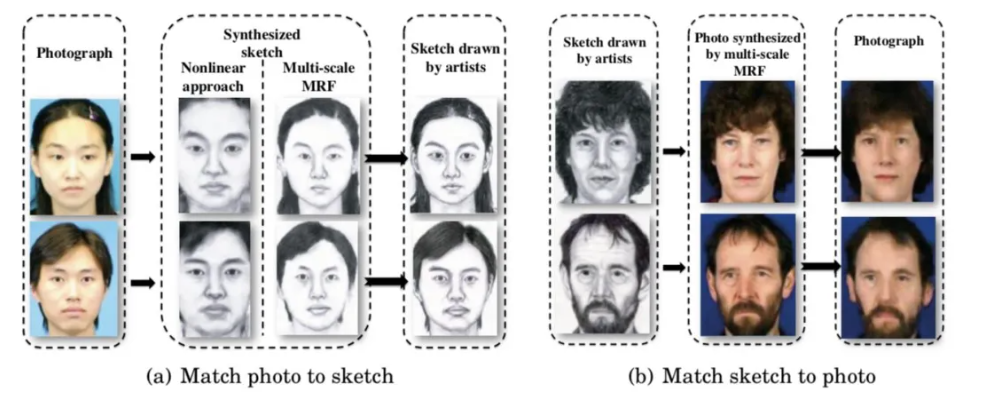
\includegraphics[width=3in]{sections/figs/s-p.png}
	\caption{\label{fig2.11} \xiaowuhao \hei Sketch-photo的转换生成}
\end{figure}
\begin{figure}[H]
	\centering
	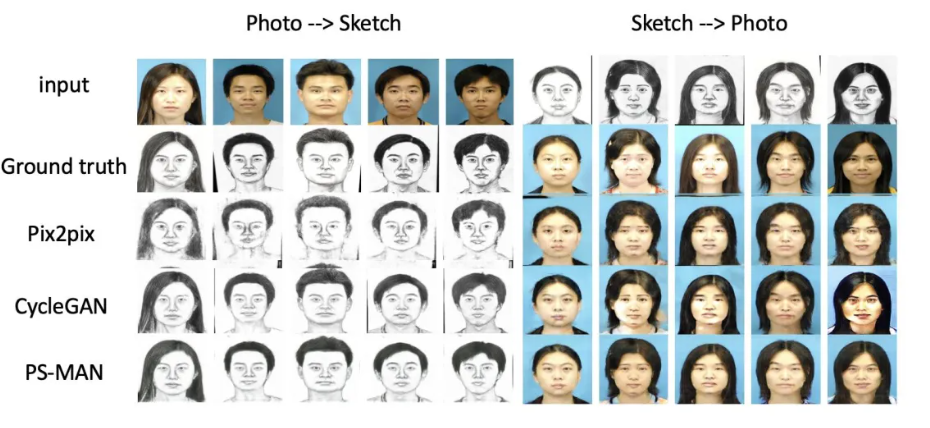
\includegraphics[width=3in]{sections/figs/gans.png}
	\caption{\label{fig2.11} \xiaowuhao \hei 利用GANs进行photo和sketch的相互转换效果图}
\end{figure}
\subsection{基于Facial landmarks的特征提取方法}
基于Facial landmarks的特征提取方法(如图3)利用
每个Facial landmark具有的视角和尺度两维参数,而其具体值由所采用的的特征提取方法决定。基于Facial landmarks的特征提取方法以固定的视角和尺度的landmark提取照片特征,以不同的视角和尺度的landmark提取漫画特征,于是每个面部地标提取到了多个跨模态指标(这是由提取漫画特征时使用了不同视角和尺度导致的)。然后利用跨模态度量学习方法(如使用距离级别的池化)来实现一个照片特征到一组漫画特征的最佳匹配,以减小照片和漫画之间视角和尺度的失调,从而达到跨模态识别的效果。
\par 下面两种特征提取方法与基于Facial landmarks的特征提取方法相结合,可以将人脸的landmark的特征信息提取,用人脸上代表性部位的特征信息对比来匹配漫画与真实图片。然而由于漫画家不同的创作风格,漫画人脸的某些特征夸张变形严重甚至出现在极不合理的位置,导致面部特征点定位困难,特征难以捕捉,这也是以下两种方法的通病。
\subsubsection{特征设计法}
特征设计法需要通过人工设计或通过学习得到在不同模态间仍然保持一致的人脸特征,同时这些特征还应满足在不同人脸间的区别度足够高,具体包括Gabor,SIFT,LBP等方法。人工设计时,这种方法的缺点在于其需要手动设计特征,虽然基于视觉神经理论,但毕竟是人为设计,难免有想当然,不妥的成分;同时在通过学习得到特征时,该方法严重依赖所给数据库,需要根据提供的数据的特点来进行设计,也就是说设计的特征不适于所有的数据集,泛化性、鲁棒性较差。当数据来源发生改变,如对RGB数据设计的特征换成了Kinect深度图像,这些特征就不一定适用,因此往往需要重新设计特征。
\subsubsection{结合CNN特征提取}
例如使用VGG-Face model,这种方法比直接利用CNN模型输出特征图的所有特征有更好的性能,比Webcaricature 只考虑单模态更能处理跨模态的表征差距,因为CNN网络强大的特征提取能力,使得这种方法性能较好。只是相对于后文提到的多任务学习方法,有些特征难以学习。

\subsection{多任务学习}
与WebCaricature等单任务学习方法相比,多任务学习方法能同时利用不同的数据训练不同的任务,如以漫画和图片作为训练数据时,多任务模型可以同时执行照片-漫画面部验证,漫画识别和照片识别,从而忽略依赖数据的噪声以学习更一般的特征。又由于该方法整合了不同的任务,所以可以学习到对于某些任务难以学习的特征。
\subsubsection{多任务学习方法}多任务学习方法分为两种:基于硬参数共享和基于软参数共享的多任务学习方法。其中,硬参数共享指的是多个任务之间共享网络的同几层隐藏层,只不过在网络的靠近输出部分开始分叉去做不同的任务;而软参数共享则是不同的任务使用不同的网络,但是不同任务的网络参数,采用距离 (L1,L2)等作为约束,鼓励参数相似化。由于不同形态的漫画和照片存在一些共同的面部特征,故使用硬参数共享的多任务学习方法是更好的选择。\subsubsection{搜索方法}多任务学习需要为每个任务设置权重,而搜索最优权重的方法主要为静态搜索与动态搜索。静态搜索中,利用实验方法手动搜索效率低,利用贪心搜索方法则费时。利用动态搜索时,若利用网络的总损失更新任务的动态权重时,容易陷入简单任务的过度训练和困难任务的不足训练。因此采用计算各个任务的损失并为具有较大损失的任务设置较大的任务权重,以重点学习困难任务。具体地,在漫画人脸照片匹配问题中,可以将漫画照片与人脸照片匹配看作主任务,将对漫画照片人物ID与真实人脸照片人物ID进行识别匹配看作另外两个子任务。将这三个任务通过最后一个共享的隐含层参数进行联系,其利用提取的任务之间的公共信息来学习任务权重。该共享隐藏层与动态权重学习模块(一个具有softmax归一化的全连接层)相连,使其生成三个任务的动态权值。该动态权重损失模块还能将各任务的损失和对应的动态权值,输入到一个新的损失函数中,以学习驱动网络专注于训练困难任务的动态权值,这样就改进了漫画人脸匹配的学习参数,使之能够有较好的效果。下图(图4)是上述自动学习生成动态权重的跨模态照片漫画识别动态多任务学习网络框架。
\end{multicols*}
\begin{figure}[H]
	\centering
	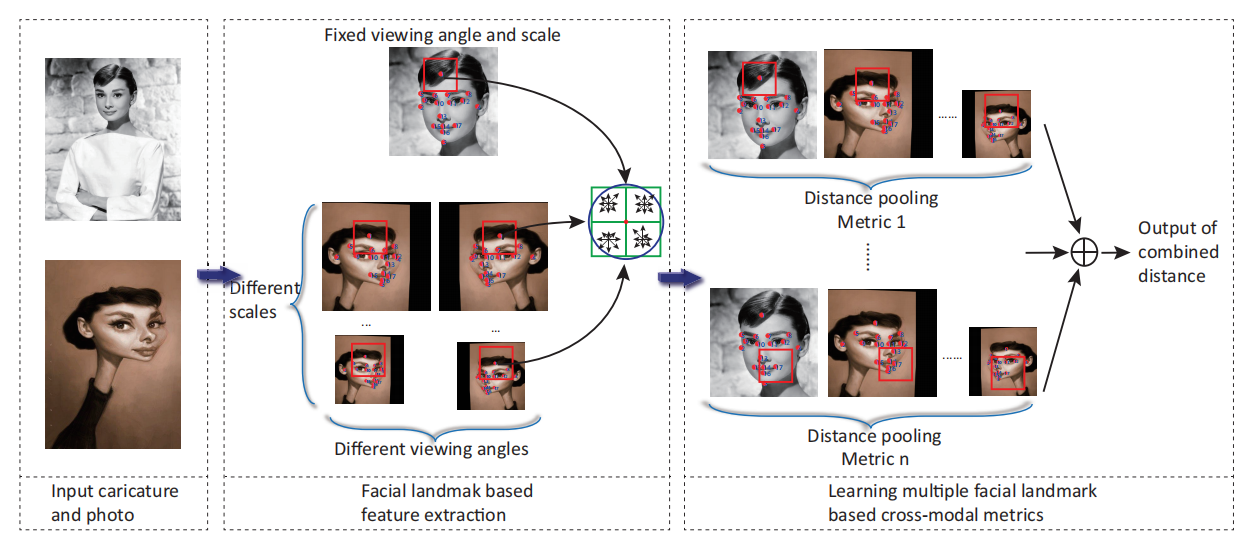
\includegraphics[width=\textwidth]{sections/figs/fl.png}
	\caption{\label{fig2.11} \xiaowuhao \hei 基于Facial landmarks的特征提取方法流程图}
\end{figure}

\begin{figure}[H]
	\centering
	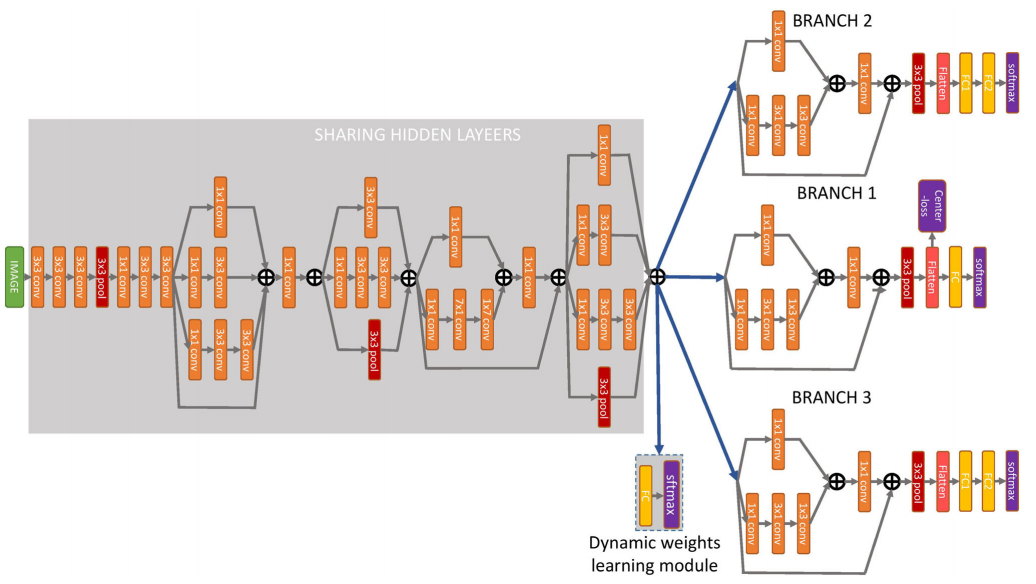
\includegraphics[width=\textwidth]{sections/figs/cnn.png}
	\caption{\label{fig2.11} \xiaowuhao \hei 自动学习生成动态权重的跨模态照片漫画识别动态多任务学习网络框架图}
\end{figure}
\begin{multicols*}{2}
~\\~\\~\\~\\~\\~\\~\\~\\
    % % \section{量的书写规则}
% 正文内容。正文、图表中的变量都要用斜体字母,对于矢量和张量使用黑斜体,只有pH采用正体;使用新标准规定的符号\cite{simonyan2014very};量的符号为单个拉丁字母或希腊字母;不能把量符号作为纯数使用;不能把化学符号作为量符号使用,代表物质的符号表示成右下标,具体物质的符号及其状态等置于与主符号齐线的圆括号中。

% 注意区分量的下标字母的正斜体:凡量符号和代表变动性数字及坐标轴的字母作下标,采用斜体字母。

% 正文中引用参考文献的标注方法,在引用处对引用的文献,按它们在论著中出现的先后用阿拉伯数字连续排序,将序号置于方括号内,并视具体情况把序号作为上角标或作为语句的组成部分。
% \subsection{单位的书写规则}
% 正文内容。单位符号无例外的采用正体字母。注意区分单位符号的大小写:一般单位符号为小写体,来源于人名的单位符号首字母大写。体积单位升的符号为大写L。
% \subsubsection{表格的规范化}
% 正文内容。表格的设计应该科学、明确、简洁,具有自明性。表格应采用三线表,项目栏不宜过繁,小表宽度小于7.5 cm,大表宽度为12~15cm 。表必须有中英文表序、表题。表中顶线与栏目线之间的部分叫项目栏,底线与栏目线之间的部分叫表身。表身中数字一般不带单位,百分数也不带百分号,应把单位符号和百分号等归并在栏目中。如果表中栏目中单位均相同,则可把共同的单位提出来标示在表格顶线上方的右端(不加“单位”二字)。表身中同一栏各行的数值应以个位(或小数点),且有效位数相同。上下左右相邻栏内的文字或数字相同时,应重复写出。

% \begin{table}[H]
% 	\xiaowuhao
% 	\centering
% 	\caption{\label{tab11} \xiaowuhao \hei 表题}
% 	\begin{tabular}{llll}
% 		\toprule
% 		Model                 & SMO+DNN & PCA+DNN & DNN   \\
% 		\midrule
% 		Accuracy              & 0.994   & 0.938   & 0.914 \\
% 		Precision             & 0.995   & 0.934   & 0.891 \\
% 		Recall                & 0.995   & 0.918   & 0.882 \\
% 		\bottomrule
% 	\end{tabular}
% \end{table}  % 第二个section(标题加内容)

    \section{不同方法的评估结果}
\subsection{数据集Webcaricature}
\begin{figure}[H]
    \centering
    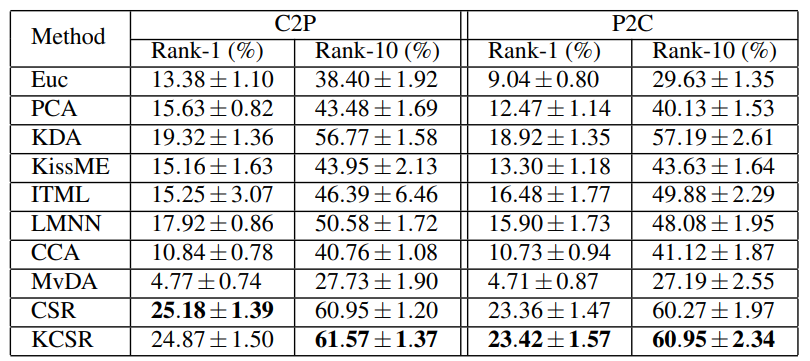
\includegraphics[width=3in]{sections/figs/eval1.png}
    \label{fig:my_label}
    \caption{\label{fig2.11} \xiaowuhao \hei 不同学习方法在C2P与P2C中的学习效果}
\end{figure}
\begin{figure}[H]
    \centering
    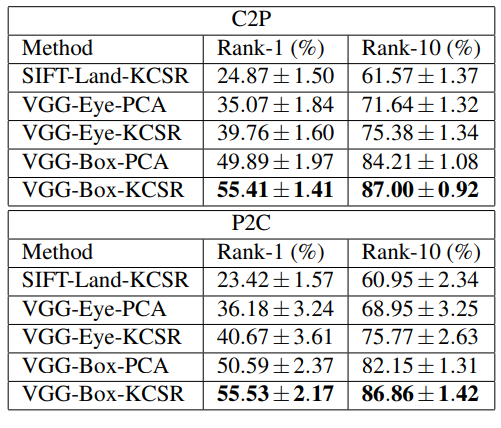
\includegraphics[width=3in]{sections/figs/eval2.png}
    \label{fig:my_label}
    \caption{\label{fig2.11} \xiaowuhao \hei 不同特征提取方法在C2P与P2C中的效果}
\end{figure}

\begin{figure}[H]
    \centering
    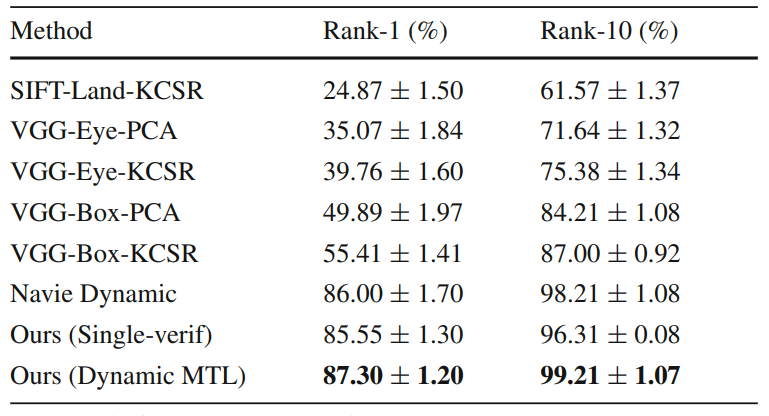
\includegraphics[width=3in]{sections/figs/eval4-1.png}
    \label{fig:my_label}
    \caption{\label{fig2.11} \xiaowuhao \hei 不同特征提取方法在C2P中的效果(与多任务学习对比)}
\end{figure}
\begin{figure}[H]
    \centering
    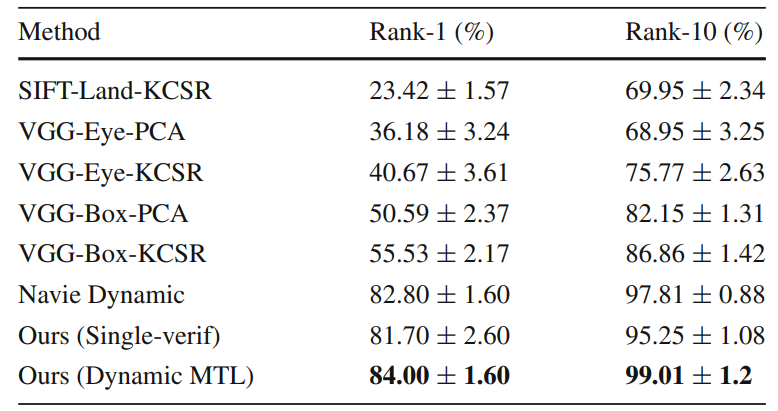
\includegraphics[width=3in]{sections/figs/eval4-2.png}
    \label{fig:my_label}
        \caption{\label{fig2.11} \xiaowuhao \hei 不同特征提取方法在P2C中的效果(与多任务学习对比)}
\end{figure}
\newpage
\subsection{数据集CaVI}
\begin{figure}[H]
    \centering
    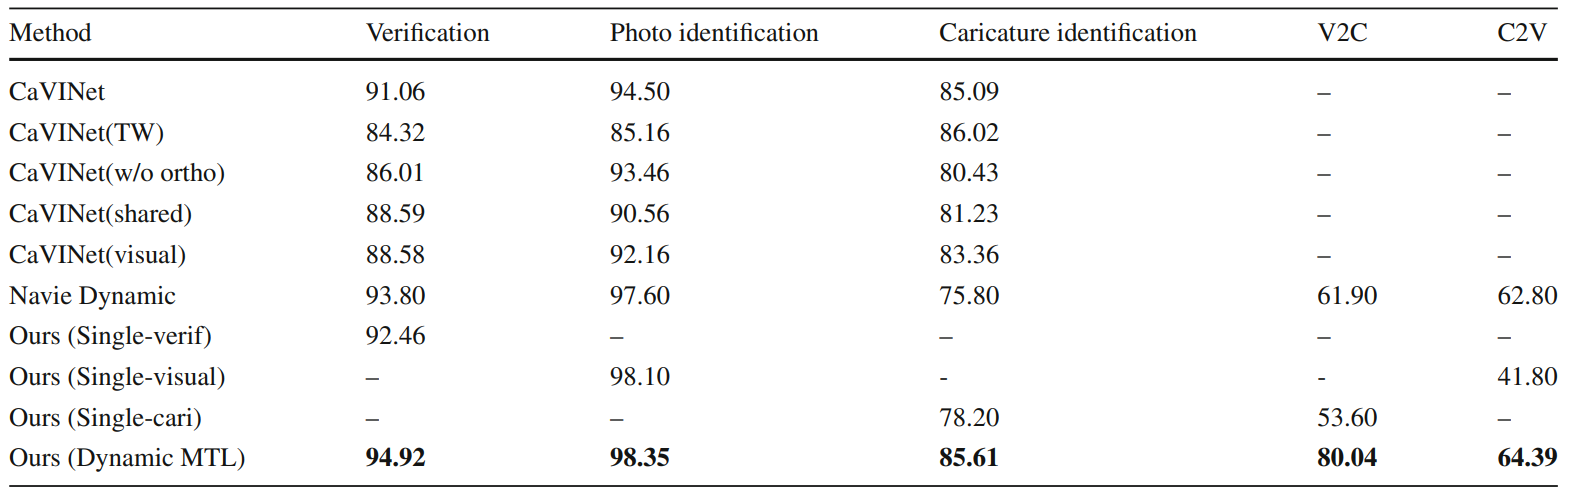
\includegraphics[width=6in]{sections/figs/eval3.png}
    \label{fig:my_label}
    \caption{\label{fig2.11} \xiaowuhao \hei 不同特征提取方法在CaVI数据集中的效果}    
\end{figure}
% \section{图}

% 正文内容。插图尽可能不用彩色图。小图宽度小于7.5 cm,大图宽度为12~15cm 。图必须有中英文图序、图题。函数图只在靠近坐标线处残留一小段标值短线,其余部分省略。加注坐标所代表的量及单位(如t/s)。标值排印在坐标外侧,紧靠标值短线的地方;标值的有效数字为3位。图中量的意义要在正文中加以解释。若有图注,靠近放在图下部,图序、图题的上方。

% % \begin{figure}[H]
% % 	\centering
% % 	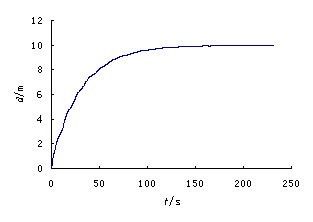
\includegraphics[width=3in]{sections/figs/template.png}
% % 	\caption{\label{fig1111} \xiaowuhao \hei 图题}
% % \end{figure}

% \section{数学符号和数学式的编排规范}
% 正文内容。变量、变动附标及函数用斜体字母表示。点、线段及弧用斜体字母表示。在特定场合中视为常数的参数也用斜体字母表示。对具有特殊定义的函数和值不变的数学常数用正体字母表示。具有特殊定义的算子也用正体字母表示。矩阵符号用大写的黑斜体字母表示,矩阵元素用白斜体字母表示。

% 公式及公式中的符号说明尽量接排以节省版面。把带有复杂上角标的指数函数$e^t$ 写成$\exp{t}$ 。公式的主体应排在同一水平线上;繁分式的主辅线要分清。长公式在运算符号后回行;长分式转行时,先将分母写成负幂指数的形式,然后转行;矩阵和行列式不能转行。矩阵元素包含式子时,每一列应以中心线上下对齐,行要左右排齐;元素为单个字母或数字时,每列应使正负号对齐。对角矩阵中对角元素所在的列应明显区分,不能上下重叠。

% 简单的和常识性的运算公式和推导过程不要列写。

% \begin{equation}
% 	\label{equ333}
% 	\begin{split}
% 		\left \{
% 		\begin{array}{ll}
% 			O_i = X &i=1 \\
% 			O_i = f_i(Z_i) & i>1 \\
% 			Z_i = g_i(O_{i-1}, W_i)
% 		\end{array}
% 		\right.
% 	\end{split}
% \end{equation}

% \begin{equation}
% 	\label{equa555}
% 	F_D = \beta \star (1-A) + (1-\beta) \star \frac{S}{D}
% \end{equation}

% \section{结束语}
% 正文内容。结论不应是正文中各段小结的简单重复,它应以正文中的实验或考察得到的现象、数据的阐述分析为依据,完整、准确、简洁地指出以下内容:1)由对研究对象进行考察或实验得到的结果所揭示的原理及其普遍性;2)研究中有无发现例外或本论文尚难以解释和解决的问题;3)与先前发表过的研究工作的异同;4)本文在理论上和实用上的意义及价值;5)进一步深入研究本课题的建议。  % 
        \section{预选方法}
通过以上调查,我们学习小组拟决定采取基于卷积神经网络(CNN)的特征提取方式,采用多任务学习方法完成此项任务。  % 
    % ...后续section

    
    % 参考文献
   %  \bibliographystyle{plain}  % 参考文献的格式
   \vspace{0.5cm}
   	\nocite{*}
    \bibliography{sections/refs.bib}  % 参考文献bib文件
\end{multicols*}
 
\end{sloppypar}
\end{document}

%%%%%%%%%%%%%%%%%%%%%%%%%%%%%%%%%%%%%%%%%%%%%%%%%%%%%%%%%%%%%%%%%%%%%%%%%%%%%%%%%%%%%%%%%%%%%%%%%%%%%%%%%%%%%%%%%%%%%%%%%%%%%%%%%%%%%%%%%%%%%%%%%%%%%%